\documentclass{beamer}
\usepackage{beamerthemesplit}
\usetheme{SPbGU}
%{CambridgeUS}
% Выпишем часть возможных стилей, некоторые из них могут содержать
% дополнительные опции
% Darmstadt, Ilmenau, CambridgeUS, default, Bergen, Madrid, AnnArbor,Pittsburg, Rochester,
% Antiles, Montpellier, Berkley, Berlin
\usepackage{pdfpages}
\usepackage{amsmath}
\usepackage{cmap} % for serchable pdf's
\usepackage[T2A]{fontenc} 
\usepackage[utf8]{inputenc}
\usepackage[english,russian]{babel}
\usepackage{indentfirst}
\usepackage{amsmath}
\usepackage{dot2texi}
\usepackage{tikz}
\usepackage{fancyvrb}
\usepackage{graphicx}
\usepackage{array}
\usepackage{subcaption}
\captionsetup{compatibility=false}
\usepackage{multimedia}
\usepackage{epstopdf}
\usepackage{multirow}
\usetikzlibrary{shapes,arrows}
% Если у вас есть логотип вашей кафедры, факультета или университета, то
% его можно включить в презентацию.

%\usefoottemplate{\vbox{}}%  \tinycolouredline{structure!25}% {\color{white}\textbf{\insertshortauthor\hfill% \insertshortinstitute}}% \tinycolouredline{structure}% {\color{white}\textbf{\insertshorttitle}\hfill}% }}

%\logo{
\includegraphics[width=1cm]{SPbGU_Logo.png}}

%[GLR-анализатор]
\title[]{О разработке инструментов статического анализа встроенных языков}
%\subtitle[студроект]{Студенческий проект}
%\institute[JetBrains]{
\institute[СПб АУ РАН]{
Санкт-Петербургский Академический Университет\\
НОЦНТ РАН}

\author[Хабибуллин Марат]{Хабибуллин Марат}

\date{22 октября 2015г.}

\begin{document}

\begin{frame}
    \begin{tabular}[c c c]{m{3cm} m{6cm} m{2,5cm}}
        \begin{center}
        
\includegraphics[width=2.5cm]{JBLogoWhite.png}
    \end{center}
    &
    Одиннадцатая независимая 
    \newline 
    научно-практическая конференция 
    \newline "Pазработка ПО 2015" 
    \newline
    22–23 (24) октября, Москва
    &
    \begin{center}
        
\includegraphics[width=2cm]{SecrLogo.png}
    \end{center}
    \\
    &&
    \end{tabular}
    \titlepage
\end{frame}

\definecolor{orange}{RGB}{179,36,31}
\begin{frame}[fragile]
	\transwipe[direction=90]
	\frametitle{Встроенные языки}
	\begin{center}
            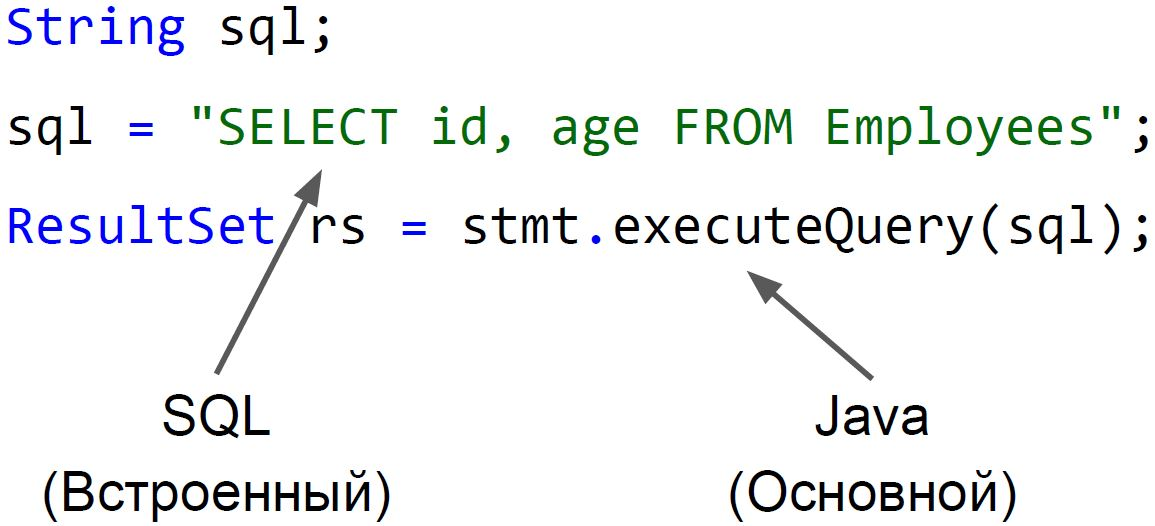
\includegraphics[width=290pt]{pictures/string_embedded_language.jpg}
        \end{center}
\end{frame}

\begin{frame}[fragile]
	\transwipe[direction=90]
	\frametitle{Примеры встраивания языков}
	\begin{itemize}
		\item SQL $\rightarrow$ Java (JDBC)
		\item JavaScript $\rightarrow$ Java (Scripting Engines)
		\item SQL $\rightarrow$ PHP (PDO)
		\item JavaScript, HTML, CSS $\rightarrow$ PHP
		\item Генераторы кода
    \end{itemize}
\end{frame}

\begin{frame}[fragile]
	\transwipe[direction=90]
	\frametitle{Проблемы}
	\begin{center}
            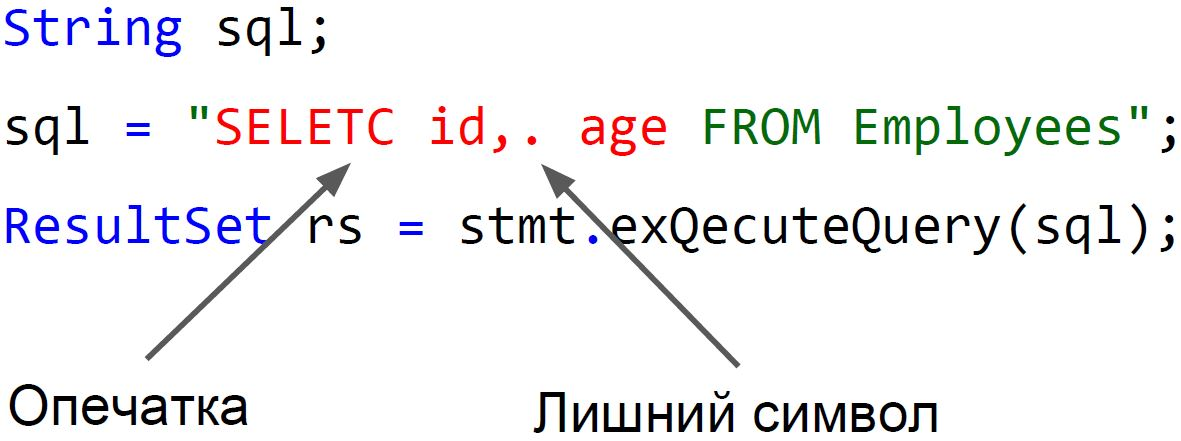
\includegraphics[width=290pt]{pictures/problems.jpg}
        \end{center}
\end{frame}

\begin{frame}[fragile]
	\transwipe[direction=90]
	\frametitle{Мотивация}
	\begin{itemize}
	    \item Поддержка в IDE 
		\begin{itemize}
			\item Подсветка синтаксиса
			\item Автодополнение
			\item Статический поиск ошибок
		\end{itemize}
	    \item Реинжиниринг
		\begin{itemize}
			\item Сбор статистики по коду на встроенном языке
			\item Автоматизированная трансформация 
		\end{itemize}
    \end{itemize}
\end{frame}

\begin{frame}[fragile]
	\transwipe[direction=90]
	\frametitle{Особенности задачи}
	\begin{center}
            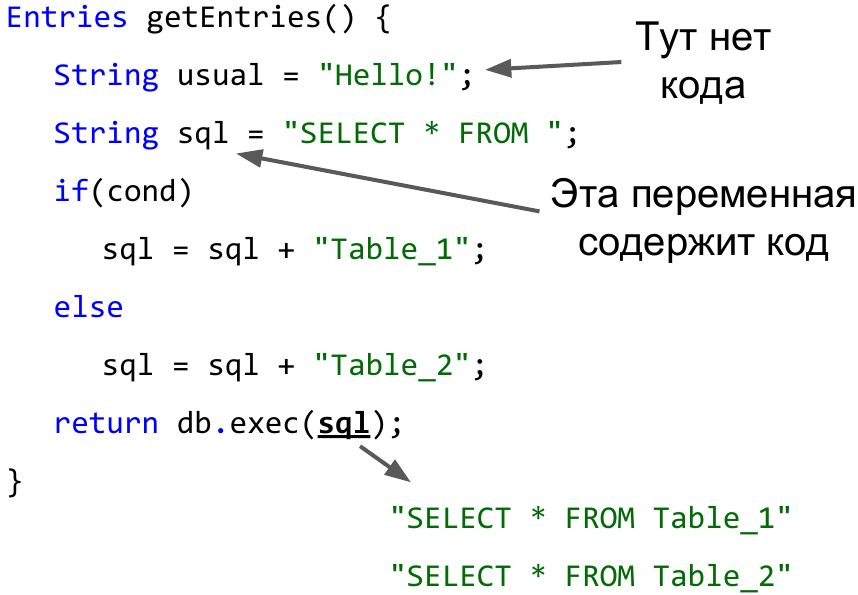
\includegraphics[width=290pt]{pictures/approximation_input.jpg}
        \end{center}
\end{frame}

\begin{frame}[fragile]
	\transwipe[direction=90]
	\frametitle{Существующие решения}
	\begin{itemize}
		\item Проверка включения языков
			\begin{itemize}
				\item Java String Analyzer ~-- регулярная аппроксимация строкового выражения
				\item PHP String Analyzer ~-- контекстно-свободная аппроксимация строкового выражения
			\end{itemize}
		\item Поддержка встроенных языков в IDE
			\begin{itemize}
				\item Varis ~-- плагин к Eclipse IDE для поддержки JS и HTML в PHP: подсветка синтаксиса, навигация
				\item IntelliLang ~-- поддержка встроенных языков в IntelliJ IDEA
				\item PHPStorm ~-- IDE для PHP с поддержкой встроенных языков
				\item Alvor ~-- плагин к Eclipse IDE для проверки встроенного в Java SQL
			\end{itemize}
	    \end{itemize}
\end{frame}

\begin{frame}[fragile]
	\transwipe[direction=90]
	\frametitle{Архитектура}
	\begin{center}
		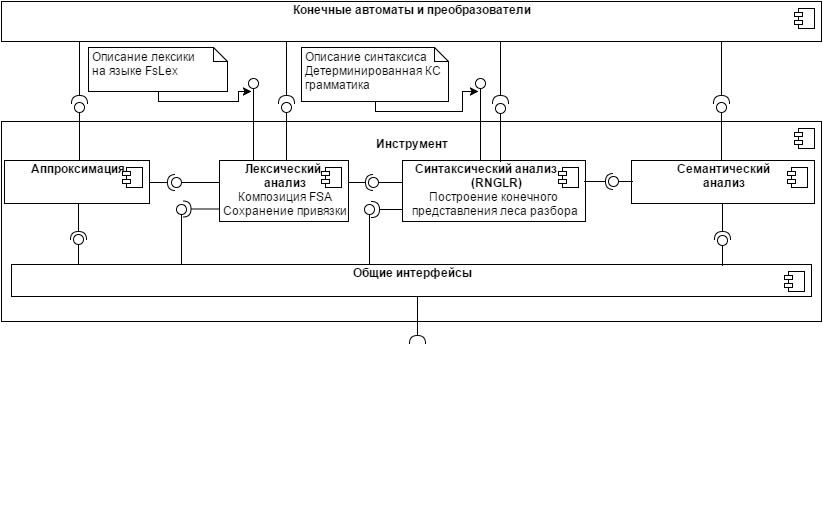
\includegraphics[width=350pt]{pictures/SELYCcomponents.jpg}
	\end{center}
\end{frame}

\begin{frame}[fragile]
	\transwipe[direction=90]
	\frametitle{Аппроксимация}
	\begin{center}
		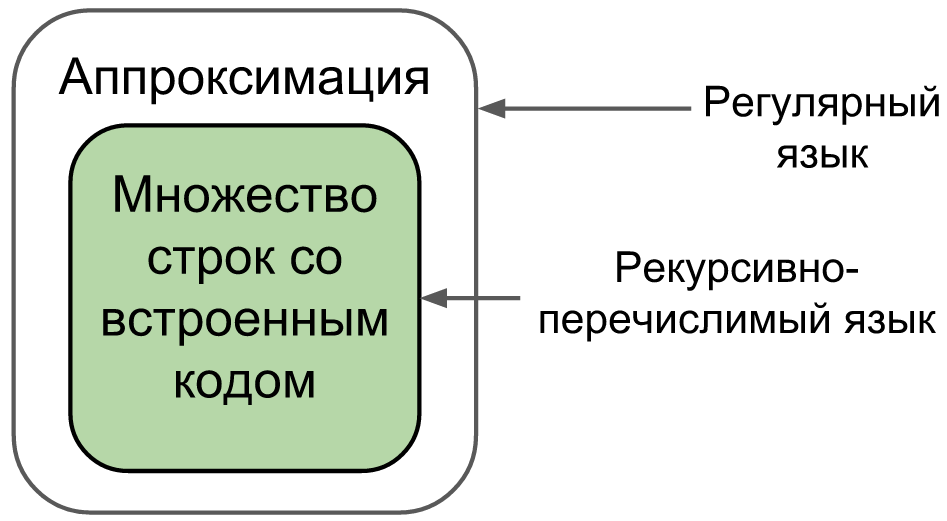
\includegraphics[width=290pt]{pictures/approximation.png}
	\end{center}
\end{frame}

\begin{frame}[fragile]
	\transwipe[direction=90]
	\frametitle{Аппроксимация: поиск строк}
	\begin{center}
            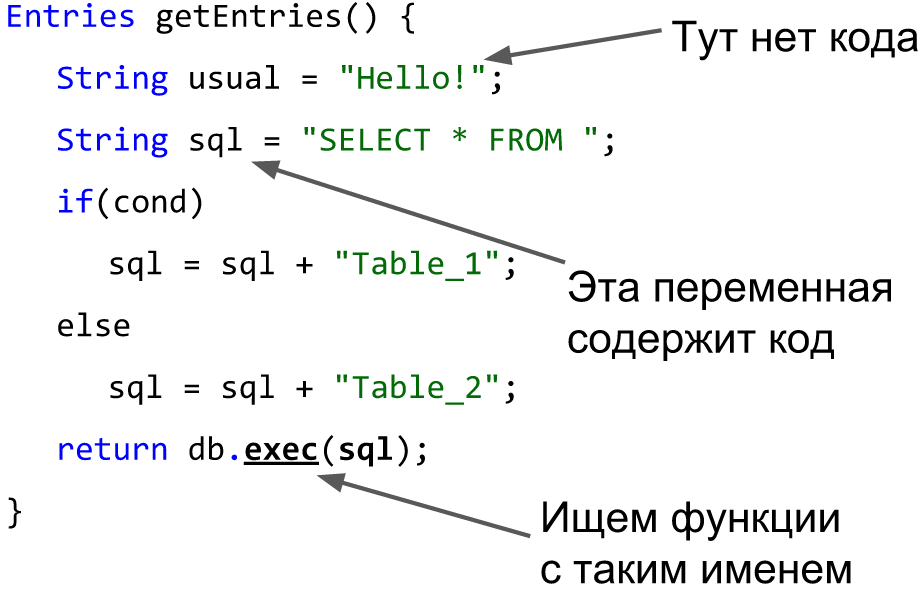
\includegraphics[width=290pt]{pictures/approximation_strings.png}
        \end{center}
\end{frame}

\begin{frame}[fragile]
	\transwipe[direction=90]
	\frametitle{Аппроксимация: граф потока управления}
	\begin{center}
            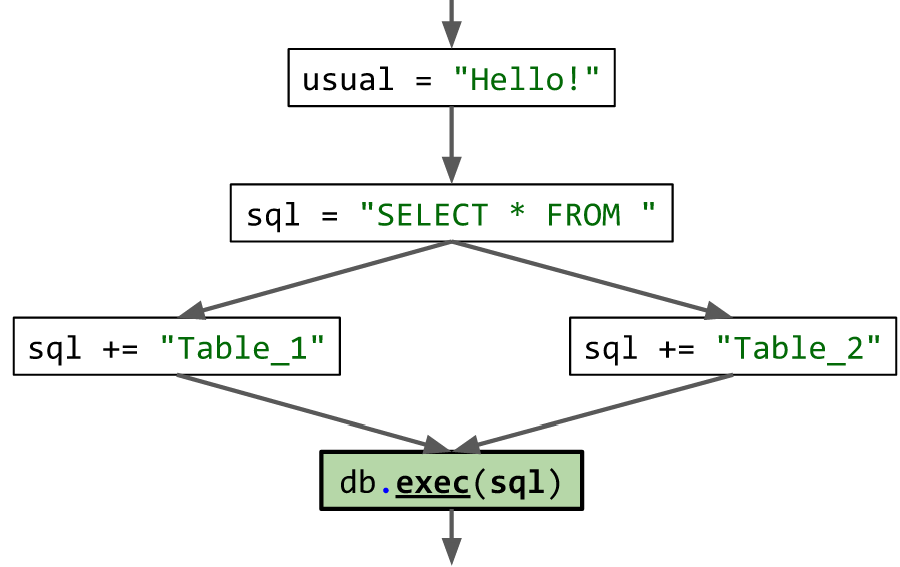
\includegraphics[width=290pt]{pictures/approximation_cfg.png}
        \end{center}
\end{frame}

\begin{frame}[fragile]
	\transwipe[direction=90]
	\frametitle{Платформа: построение аппроксимации}
	\begin{center}
            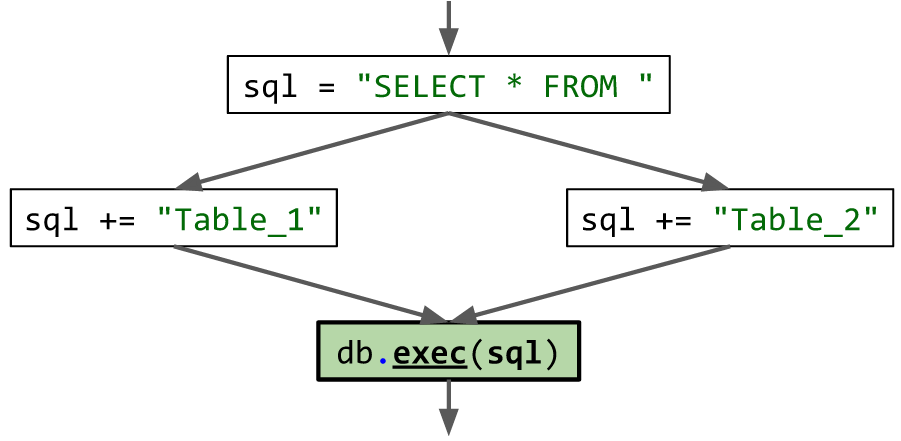
\includegraphics[width=290pt]{pictures/approximation_result.png}
        \end{center}
\end{frame}

\begin{frame}[fragile]
	\transwipe[direction=90]
	\frametitle{Лексический анализ}
	\begin{itemize}
	    	\item Автомат над строками $\rightarrow$ автомат над токенами
    		\begin{itemize}
			\item Токен ~-- идентификатор + конечный автомат
			\item Привязка лексических единиц к исходному коду
	    	\end{itemize}
		\begin{center}
			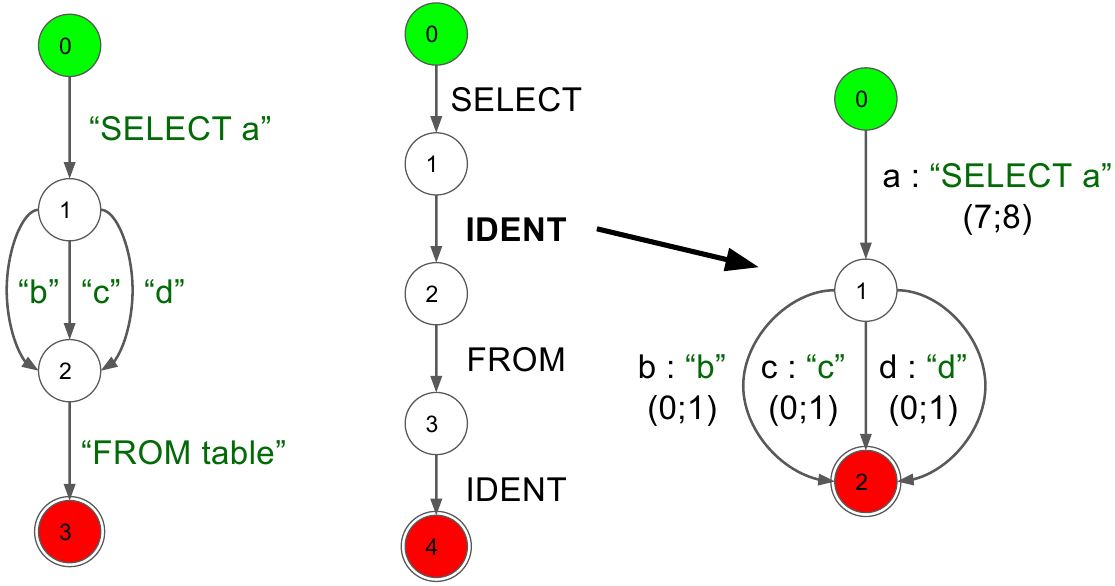
\includegraphics[width=290pt]{pictures/lexing.jpg}
		\end{center}
        \end{itemize}
\end{frame}

\begin{frame}[fragile]
	\transwipe[direction=90]
	\frametitle{Синтаксический анализ}

	    \begin{tabular}{p{5.8cm} p{6.2cm}}
		\underline{Грамматика:}& \underline{Результат (SPPF):}
		\vspace{-20pt}
		\\
		\vspace{-20pt}
		
		$$
		\begin{array}{crcl}
		(0)& start\_rule &::=& s \\
		(1)& s & ::= & \mbox{\texttt{LBR }} s \mbox{\texttt{ RBR }} s\\
		(2)& s & ::= &\varepsilon
		\end{array}
		$$
		&
		\\      
		\underline{Вход:} \vspace{10pt}&
		\\
		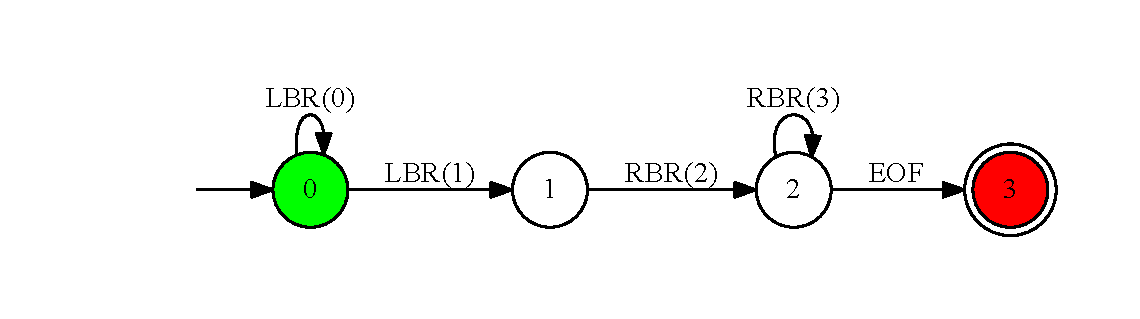
\includegraphics[width=170pt]{pictures/parser_input.pdf}
		& \multirow{-9}*{\!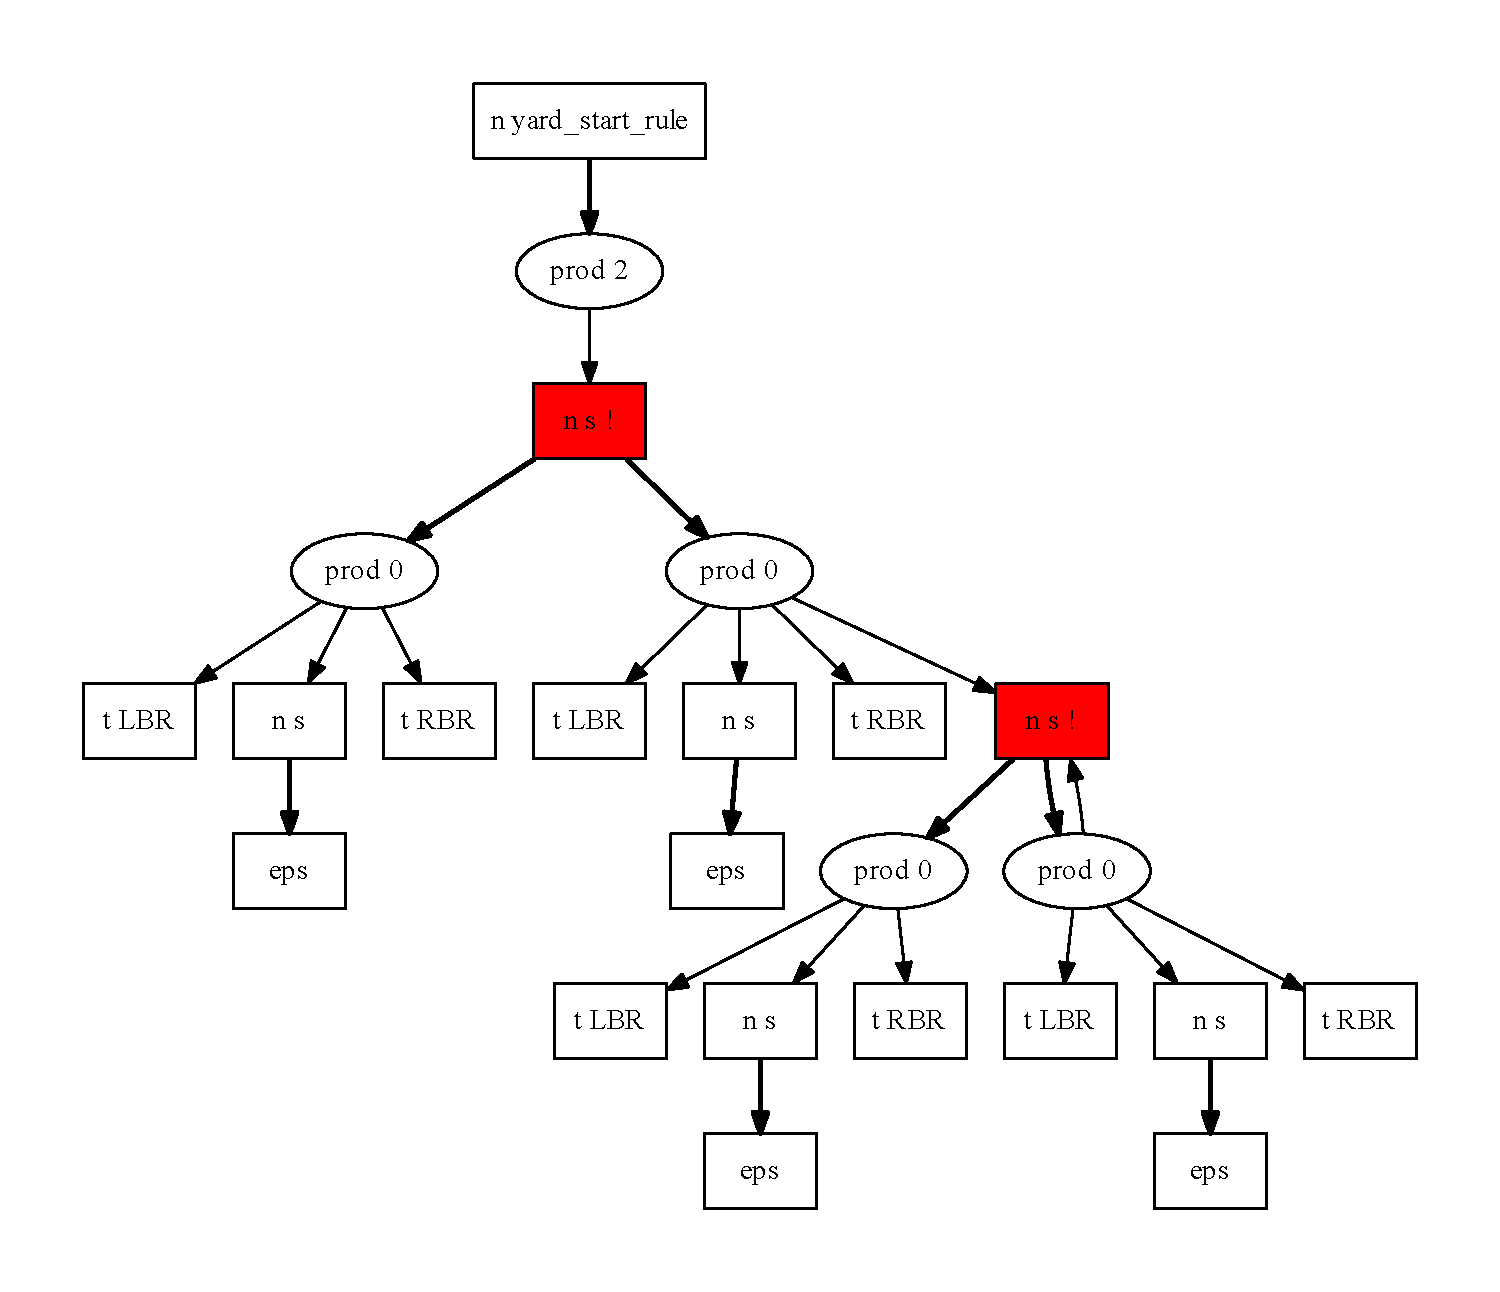
\includegraphics[width=168pt]{pictures/parser_output.pdf}}
	\end{tabular}

\end{frame}

\begin{frame}[fragile]
	\transwipe[direction=90]
	\frametitle{Реализация}

	\begin{itemize}
		\item YaccConstructor ~-- платформа для исследований в области синтаксического анализа
		\item Наша платформа ~-- часть YaccConstructor
			\begin{itemize}
				\item Генератор абстрактных лексических анализаторов
				\item Генератор абстрактных синтаксических анализаторов
				\item Модульная архитектура для языковых расширений
			\end{itemize}
		\item Плагин для ReSharper
			\begin{itemize}
				\item Расширяемая архитектура, позволяющая легко поддержать любой встроенный язык
				\item Основной язык должен поддерживаться в ReSharper
				\item Анализаторы SQL и Calc, встроенных в C\# и JavaScript
			\end{itemize}
	\end{itemize}
\end{frame}

\begin{frame}[fragile]
	\transwipe[direction=90]
	\frametitle{Демонстрация}
	\begin{center}
            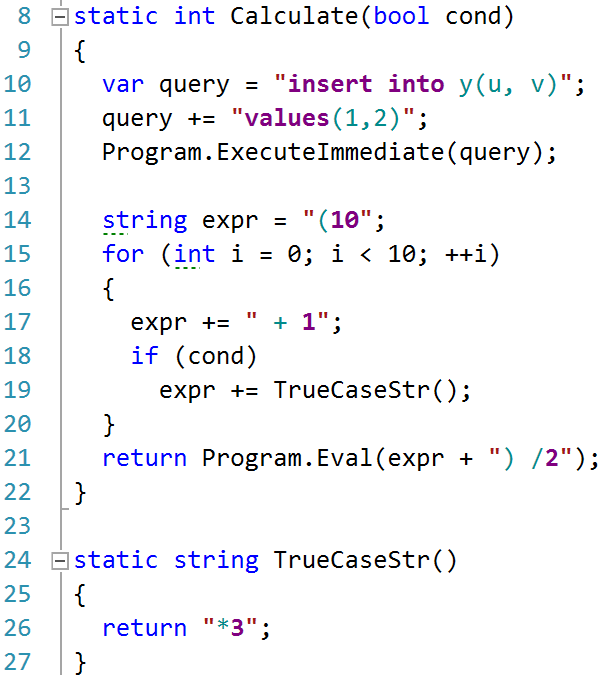
\includegraphics[width=200pt]{pictures/sql_and_calc_cycle.PNG}
        \end{center}
\end{frame}

\begin{frame}[fragile]
	\transwipe[direction=90]
	\frametitle{Демонстрация}
	\begin{center}
            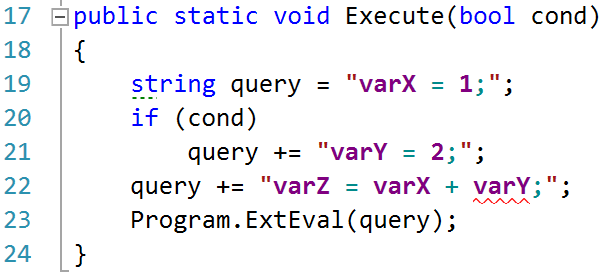
\includegraphics[width=290pt]{pictures/Undefined_variable.PNG}
        \end{center}
\end{frame}

\begin{frame}
	\transwipe[direction=90]
	\frametitle{Информация о проекте}
	\begin{itemize}
		\item Контакты: 
        \begin{itemize}
	 \item Хабибуллин Марат: maratx387@gmail.com
            \item Иванов Андрей: ivanovandrew2004@gmail.com
            \item Григорьев Семён: Semen.Grigorev@jetbrains.com
        \end{itemize}
		\item Исходный код YaccConstructor: \href{https://github.com/YaccConstructor}{https://github.com/YaccConstructor}		
		\item Google+ сообщество: \href{https://plus.google.com/u/0/communities/102842370317111619055}{https://plus.google.com/u/0/communities/102842370317111619055}
	\end{itemize}
\end{frame}

\end{document}
